\documentclass[]{article}
\usepackage{lmodern}
\usepackage{amssymb,amsmath}
\usepackage{ifxetex,ifluatex}
\usepackage{fixltx2e} % provides \textsubscript
\ifnum 0\ifxetex 1\fi\ifluatex 1\fi=0 % if pdftex
  \usepackage[T1]{fontenc}
  \usepackage[utf8]{inputenc}
\else % if luatex or xelatex
  \ifxetex
    \usepackage{mathspec}
  \else
    \usepackage{fontspec}
  \fi
  \defaultfontfeatures{Ligatures=TeX,Scale=MatchLowercase}
\fi
% use upquote if available, for straight quotes in verbatim environments
\IfFileExists{upquote.sty}{\usepackage{upquote}}{}
% use microtype if available
\IfFileExists{microtype.sty}{%
\usepackage{microtype}
\UseMicrotypeSet[protrusion]{basicmath} % disable protrusion for tt fonts
}{}
\usepackage[margin=1in]{geometry}
\usepackage{hyperref}
\hypersetup{unicode=true,
            pdftitle={Aplicación de Procesamiento de Lenguaje Natural en las ciencias sociales. Detección automática de tópicos en letras de tango},
            pdfauthor={Germán Rosati (CONICET - IDAES/UNSAM - PIMSA)},
            pdfborder={0 0 0},
            breaklinks=true}
\urlstyle{same}  % don't use monospace font for urls
\usepackage{longtable,booktabs}
\usepackage{graphicx}
% grffile has become a legacy package: https://ctan.org/pkg/grffile
\IfFileExists{grffile.sty}{%
\usepackage{grffile}
}{}
\makeatletter
\def\maxwidth{\ifdim\Gin@nat@width>\linewidth\linewidth\else\Gin@nat@width\fi}
\def\maxheight{\ifdim\Gin@nat@height>\textheight\textheight\else\Gin@nat@height\fi}
\makeatother
% Scale images if necessary, so that they will not overflow the page
% margins by default, and it is still possible to overwrite the defaults
% using explicit options in \includegraphics[width, height, ...]{}
\setkeys{Gin}{width=\maxwidth,height=\maxheight,keepaspectratio}
\IfFileExists{parskip.sty}{%
\usepackage{parskip}
}{% else
\setlength{\parindent}{0pt}
\setlength{\parskip}{6pt plus 2pt minus 1pt}
}
\setlength{\emergencystretch}{3em}  % prevent overfull lines
\providecommand{\tightlist}{%
  \setlength{\itemsep}{0pt}\setlength{\parskip}{0pt}}
\setcounter{secnumdepth}{0}
% Redefines (sub)paragraphs to behave more like sections
\ifx\paragraph\undefined\else
\let\oldparagraph\paragraph
\renewcommand{\paragraph}[1]{\oldparagraph{#1}\mbox{}}
\fi
\ifx\subparagraph\undefined\else
\let\oldsubparagraph\subparagraph
\renewcommand{\subparagraph}[1]{\oldsubparagraph{#1}\mbox{}}
\fi

%%% Use protect on footnotes to avoid problems with footnotes in titles
\let\rmarkdownfootnote\footnote%
\def\footnote{\protect\rmarkdownfootnote}

%%% Change title format to be more compact
\usepackage{titling}

% Create subtitle command for use in maketitle
\providecommand{\subtitle}[1]{
  \posttitle{
    \begin{center}\large#1\end{center}
    }
}

\setlength{\droptitle}{-2em}

  \title{Aplicación de Procesamiento de Lenguaje Natural en las ciencias
sociales. Detección automática de tópicos en letras de tango}
    \pretitle{\vspace{\droptitle}\centering\huge}
  \posttitle{\par}
    \author{Germán Rosati (CONICET - IDAES/UNSAM - PIMSA)}
    \preauthor{\centering\large\emph}
  \postauthor{\par}
    \date{}
    \predate{}\postdate{}
  

\begin{document}
\maketitle

\subsection{Introducción}\label{introducciuxf3n}

Es una obviedad decirlo, pero el lenguaje es parte integrante de la
sociedad. Independientemente de posiciones idealistas o materialistas al
respecto, lo cierto es que buena parte de las interacciones a lo largo y
a lo ancho de la estructura social, se encuentran mediadas por el
lenguaje y tiene como producto una gran cantidad de ``textos''``, muchos
de los cuales no son escritos, pero muchos otros sí.

Desde las ciencias sociales se ha hecho énfasis en esta idea, llegando a
extremos teóricos y metodológicos y afirmaciones temerarias tales como
que la sociedad ES un texto o que la cultura puede ser interpretada de
la misma forma y con las mismas herramientas con que se aborda un texto
literario. Uno de los referentes más relevantes de de la antropología
interpretativa escribe en uno de sus textos más famosos:

\begin{quote}
The culture of a people is an ensemble of texts, themselves ensembles,
which the anthropologist strains to read over the shoulders of those to
whom they properly belong. (Geertz, 1974)
\end{quote}

Este enfoque ha ido acompañado de posiciones metodológicas más bien
ligadas al análisis literario o filosófico: los métodos vinculados a la
deconstrucción y a la hermenéutica constituyen algunos ejemplos. En la
cita anterior resalta un requisito metodológico importante de este
conjunto de enfoques: el objeto (la cultura) debe ser tratado por
investigador como si fuera un texto, lo cual pone en un lugar central a
la operación de ``interpretación''. Así, las herramientas y técnicas
metodológicas de las que se suele echar mano en este tipo de enfoques se
encuentran más vinculadas al análisis literario, al análisis del
discurso y a métodos que buscan la comprensión del detalle y el
contexto. Dichos enfoques han sido objeto de diversas críticas (Reynoso,
2007). No es objeto del presente trabajo evaluar dichas críticas y solo
se remarcará un aspecto relevante a tener en cuenta: en términos
generales, las posturas interpretativistas tienden a poner el eje en la
capacidad subjetiva del investigador para realizar la interpretación.
Esto hace que buena parte de las investigaciones realizadas bajo este
tipo de marcos teóricos presenten (potencialmente) una relativa falta de
sistematicidad metodológica y que el peligro de la imposibilidad de
replicación de sus resultados esté siempre latente.

Las técnicas abordadas en este artículo pueden ser de utilidad a las
ciencias sociales dado que permiten realizar una sistematización (y,
eventualmente, lograr un cierto grado de automatización) de los diversos
pasos de preprocesamiento de un texto y habilitan la aplicación de
métodos cuantitativos de análisis para una amplia diversidad de tareas
(clasificación de textos, detección de temas y tópicos, etc.).

Un segundo punto a considerar en este tipo de abordajes se vincula al
problema de la escala. Existen algunas aproximaciones basadas en la
tradición hermenéutica que buscan llegar a un grado más alto de
sistematización de los procesos y etapas del análisis. El Qualitative
Content Analysis (Hsieh \& Shannon, 2005), por ejemplo, busca
sistematizar las diversas etapas y decisiones metodológicas en el
proceso de análisis de datos no estructurados textuales. El problema que
surge aquí es la escala: la transcripción y codificación manual de
corpus textuales limita fuertemente el tamaño de los corpus a analizar.

Una vez más, las técnicas de \emph{Text Mining} y \emph{Natural Language
Processing} abren la posibilidad de escalar el trabajo de forma
eficiente. En lugar de leer cada uno de los textos de un corpus, tarea
que rápidamente se vuelve imposible, las técnicas de minería de texto
permiten analizar de forma automática corpus de escalas notablemente
grandes.

El presente trabajo tiene como objetivo general discutir algunas
aproximaciones metodológicas al análsis automático de textos y presentar
algunas de las potencialidades que tienen en el trabajo cotidiano de las
ciencias sociales a partir de su aplicacion a un caso de estudio
concreto: el análisis de los temas en un corpus de 6.200 letras de
tango. Particularmente, nos centraremos en la discusión de algunos
aspectos del flujo de trabajo para el análisis de texto y en la
aplicación y discusión de una técnica específica para resolución de un
problema general del Procesamiento de Lenguaje Natural: el modelo
\emph{Latent Dirichlet Allocation} (LDA) para la detección de tópicos en
un corpus.

\subsection{2. Antecedentes metodológicos en el análisis de letras de
tango}\label{antecedentes-metodoluxf3gicos-en-el-anuxe1lisis-de-letras-de-tango}

El análisis de contenido en letras de tango no es un tema nuevo y existe
una gran cantidad de literatura al respecto. Es importante tener en
cuenta que el objetivo central del artículo es ilustrar la aplicación de
un proceso de trabajo y de algunas técnicas de análisis vinculadas al
campo del NLP. Se centra, entonces, en la dimensión metodológica del
problema. Es por ello que los textos reseñados esta sección son
ilustrativos en esa dimensión.

Un abordaje común es el rastreo de un tópico o problema particular a lo
largo de un corpus textual. En el caso del análisis de letras de tango
un tópico habitual se vincula a los estudios de género. Irene López
(2010) aborda cuáles son las representaciones que se hacen de las
mujeres sobre un corpus de aproximadamente 10 letras de tango de
diferentes épocas y autores. A su vez, Juan Gasparri (2011) busca
identificar las formas en que las masculinidades (particularmente, la
del ``guapo'' en sus diversas construcciones) aparecen en un corpus de
alrededor de 16 textos. También, teniendo como eje la problemática de
género, Carolina Marchese (2007) rastrea la temática amorosa y el sesgo
sentimental en aproximadamente 30 tangos de fines del siglo XIX y
principios del XX\footnote{El tamaño de los corpus está referido a la
  cantidad de textos que citan o mencionan los diferentes autores en
  cada uno de los trabajos citados. Lógicamente, es razonable asumir que
  solamente se cita una fracción -desconocida- de los textos analizados.}.

A su vez, otros textos tienen un enfoque más amplio y tratan de relevar
una mayor cantidad de temas o problemas en las letras de tango. Así,
Lucía Willenpart(2011) rastrea e identifica algunos temas comunes: el
amor, el duelo amoroso, la mujer, la madre, el tango mismo, etc.

Por otro lado, Cantón (1972) se pregunta por los objetos y sujetos de
los tangos cantados por Carlos Gardel. Este estudio tiene un carácter
cuantitativo, por lo cual analiza un corpus significativamente más
grande que los anteriores: alrededor de 100 tangos.

De esta forma, en términos metodológicos es posible identificar tres
rasgos de los textos reseñados:

\begin{enumerate}
\def\labelenumi{\arabic{enumi}.}
\tightlist
\item
  no aparecen criterios claros para la confección del corpus, con todos
  los potenciales segos y problemas que esto conlleva
\item
  el tamaño de los corpus es entre pequeño (10 tangos) y mediano (100
  tangos)
\item
  con la excepción del texto de Cantón (Cantón, 1972), los textos son
  abordados a partir del rastreo de un tópico o pregunta particular en
  profundidad, privilegiándose un análisis interpretativo del contenido.
\end{enumerate}

\subsection{3. Construcción del corpus y flujo de
trabajo}\label{construcciuxf3n-del-corpus-y-flujo-de-trabajo}

A los efectos de ilustrar un caso de aplicación de este tipo de
técnicas, se presentará un flujo de trabajo clásico aplicado a la
detección de tópicos en un corpus textual de letras de tango. El corpus
fue construido a partir de un proceso de web scraping\footnote{El
  \emph{scraping}-literalmente, ``raspado'' o ``rascado'' consiste en la
  descarga y formateo de la información disponible en sitios web,
  información que generalmente no se encuentra en condiciones de ser
  trabajada de forma estadística (Mitchell, 2015).} Se descargaron todas
las letras de tango disponibles en el sitio
\href{www.todotango.com}{todo tango}.

Además de las letras se descargó información accesoria sobre el tango en
cuestión. Para ello se confeccionaron dos web crawlers
sencillos\footnote{El código puede ser consultado en nuestro repositorio
  \url{http://www.github/gefero}.}.

El corpus final consiste en alrededor de 5700 letras de tango, agrupadas
en un dataset con la siguiente estructura:

\textbf{Tabla 1. Ejemplo de base de datos utilizada}

\begin{longtable}[]{@{}llllll@{}}
\toprule
\begin{minipage}[b]{0.09\columnwidth}\raggedright\strut
Título\strut
\end{minipage} & \begin{minipage}[b]{0.07\columnwidth}\raggedright\strut
Ritmo\strut
\end{minipage} & \begin{minipage}[b]{0.06\columnwidth}\raggedright\strut
Año\strut
\end{minipage} & \begin{minipage}[b]{0.11\columnwidth}\raggedright\strut
Compositor\strut
\end{minipage} & \begin{minipage}[b]{0.11\columnwidth}\raggedright\strut
Autor\strut
\end{minipage} & \begin{minipage}[b]{0.38\columnwidth}\raggedright\strut
Letra\strut
\end{minipage}\tabularnewline
\midrule
\endhead
\begin{minipage}[t]{0.09\columnwidth}\raggedright\strut
A bailar\strut
\end{minipage} & \begin{minipage}[t]{0.07\columnwidth}\raggedright\strut
Tango\strut
\end{minipage} & \begin{minipage}[t]{0.06\columnwidth}\raggedright\strut
1943\strut
\end{minipage} & \begin{minipage}[t]{0.11\columnwidth}\raggedright\strut
D. Federico\strut
\end{minipage} & \begin{minipage}[t]{0.11\columnwidth}\raggedright\strut
H. Expósito\strut
\end{minipage} & \begin{minipage}[t]{0.38\columnwidth}\raggedright\strut
a bailar a bailar que la orquesta se va\ldots{}\strut
\end{minipage}\tabularnewline
\begin{minipage}[t]{0.09\columnwidth}\raggedright\strut
\ldots{}\strut
\end{minipage} & \begin{minipage}[t]{0.07\columnwidth}\raggedright\strut
\ldots{}\strut
\end{minipage} & \begin{minipage}[t]{0.06\columnwidth}\raggedright\strut
\ldots{}\strut
\end{minipage} & \begin{minipage}[t]{0.11\columnwidth}\raggedright\strut
\ldots{}\strut
\end{minipage} & \begin{minipage}[t]{0.11\columnwidth}\raggedright\strut
\ldots{}\strut
\end{minipage} & \begin{minipage}[t]{0.38\columnwidth}\raggedright\strut
\ldots{}\strut
\end{minipage}\tabularnewline
\begin{minipage}[t]{0.09\columnwidth}\raggedright\strut
Malena\strut
\end{minipage} & \begin{minipage}[t]{0.07\columnwidth}\raggedright\strut
Tango\strut
\end{minipage} & \begin{minipage}[t]{0.06\columnwidth}\raggedright\strut
1941\strut
\end{minipage} & \begin{minipage}[t]{0.11\columnwidth}\raggedright\strut
L. Demare\strut
\end{minipage} & \begin{minipage}[t]{0.11\columnwidth}\raggedright\strut
H. Manzi\strut
\end{minipage} & \begin{minipage}[t]{0.38\columnwidth}\raggedright\strut
malena canta el tango como ninguna\ldots{}\strut
\end{minipage}\tabularnewline
\begin{minipage}[t]{0.09\columnwidth}\raggedright\strut
Zurdo\strut
\end{minipage} & \begin{minipage}[t]{0.07\columnwidth}\raggedright\strut
Tango\strut
\end{minipage} & \begin{minipage}[t]{0.06\columnwidth}\raggedright\strut
S/D\strut
\end{minipage} & \begin{minipage}[t]{0.11\columnwidth}\raggedright\strut
A. Pontier\strut
\end{minipage} & \begin{minipage}[t]{0.11\columnwidth}\raggedright\strut
F. Silva\strut
\end{minipage} & \begin{minipage}[t]{0.38\columnwidth}\raggedright\strut
era del tiempo lindo que siempre es antes\ldots{}\strut
\end{minipage}\tabularnewline
\bottomrule
\end{longtable}

Si bien el resto de la información recolectada podría ser utilizada, en
este trabajo y para poder ilustrar de forma más clara el trabajo sobre
texto crudo, nos centraremos solamente en el campo que contiene las
letras. Ese será el corpus final.

Se trata de un caso típico de datos no estructurados: las letras
constituyen texto libre y no parece respetarse la estructura tripartita
del dato. Las filas sí representan una unidad (los tangos) pero no
tenemos atributos, o en todo caso, solamente tenemos un atributo, la
letra. El primer paso, entonces, poder pasar de esta representación no
estructurada a una estructurada. Esta representación tendrá como objeto
reducir la complejidad del texto, dado que ``el lenguage es complejo.
Pero no toda su complejidad es necesaria para analizar un texto de forma
efectiva'' (Grimmer \& Stewart, 2013).

\subsubsection{\texorpdfstring{3.1 Modelo \emph{BoW} (\emph{Bag of
words})}{3.1 Modelo BoW (Bag of words)}}\label{modelo-bow-bag-of-words}

Para llegar a esa representación estructurada\footnote{Vale destacar que
  el flujo de trabajo descripto a continuación es uno posible -y
  bastante común-, pero de ninguna manera el único, ni necesariamente el
  ``mejor'' en términos absoltos. El flujo y las operaciones contenidas
  en el mismo deberán ser revisadas para cada problema
  particular(Grimmer \& Stewart, 2013).}, será necesario pensar en una
estructura de datos acorde a las necesidades del análisis. En primer
lugar, la unidad de análisis serán los tangos individuales, por lo cual,
cada fila en la matriz final será un tango. A su vez, la representación
a utilizar será la siguiente: cada columna consistirá en un término
\(t\) del vocabulario general \(V\) del corpus \(C\). Finalmente, cada
celda estará constituida por el conteo crudo de ocurrencias de cada
palabra (columna) en cada documento (fila). Esta representación es la
que se denomina \emph{Bag of Words} o ``bolsa de palabras'' y se dispone
en una Matriz de Frecuencias de Términos (\(TFM\), por sus siglas en
inglés).

Por ejemplo, para dos de los tangos analizados esta matriz tomaría la
siguiente forma:

\textbf{Tabla 2. Ejemplo de matriz de frecuencia de términos cruda}

\begin{longtable}[]{@{}lllllllllllll@{}}
\toprule
Letra & agua & blanda & cartel & cruel & el & en & era & la & manda &
mas & propaganda & que\tabularnewline
\midrule
\endhead
Cruel en el cartel la propaganda manda cruel en el cartel & 0 & 0 & 2 &
2 & 2 & 2 & 0 & 1 & 1 & 0 & 1 & 0\tabularnewline
Era más blanda que el agua que el agua blanda & 2 & 2 & 0 & 0 & 2 & 0 &
1 & 0 & 0 & 1 & 0 & 2\tabularnewline
\bottomrule
\end{longtable}

Puede verse que al construir esta matriz la información sobre el orden
de las palabras se ha perdido. En efecto, el orden de las columnas es
ahora arbitrario (en este caso, lexicográfico) y no respeta la
estructura secuencial de las palabras en un texto. Esta es una
simplificación importante del modelo \(BoW\). Esta limitación puede
subsanarse parcialmente generando una TFM de bi-gramas (pares de
palabras), tri-gramas (tripletas de palabras) o n-gramas. El costo es un
crecimiento exponencial en la dimensionalidad de la TFM

Debe tenerse en cuenta que esta matriz se construye sobre el vocabulario
\(V\) , o sea el total de términos únicos sobre el corpus \(C\). Así,
\(V\) incluiría a priori signos de puntuación, diferentes conjugaciones
de verbos, sustantivos en singular o plural, etc. Esto hace que el
vocabulario ``crudo'' de \(C\) tienda a ser demasiado grande. Es por
ello que, en la etapa de preprocesamiento del texto se utilizan algunas
técnicas para reducir la complejidad y la extensión de \(V\).

Un primer paso simple es la eliminación de lo que suelen denominarse
stopwords, básicamente artículos, preposiciones, conectores, etc. La
lógica detrás de esta eliminación es que estas palabras se encuentran en
todos los documentos \(d\) de \(C\) por lo cual aportan poca información
acerca de su contenido.

\textbf{Tabla 3. Ejemplo de matriz de frecuencia de términos sin
stopwords}

\begin{longtable}[]{@{}llllllll@{}}
\toprule
Letra & agua & blanda & cartel & cruel & manda & mas &
propaganda\tabularnewline
\midrule
\endhead
Cruel en el cartel la propaganda manda cruel en el cartel & 0 & 0 & 2 &
2 & 1 & 0 & 1\tabularnewline
Era más blanda que el agua que el agua blanda & 2 & 2 & 0 & 0 & 0 & 1 &
0\tabularnewline
\bottomrule
\end{longtable}

A partir de la eliminación de las \emph{stopwords} se obtiene en la
tabla 3 una representación más resumida de la información contenida en
\(C\). No obstante, ésta no es la única operación disponible para
reducir la complejidad de \(C\).

\subsubsection{\texorpdfstring{3.2 Normalización de términos:
\emph{stemming} y
lematización}{3.2 Normalización de términos: stemming y lematización}}\label{normalizaciuxf3n-de-tuxe9rminos-stemming-y-lematizaciuxf3n}

El paso siguiente consiste en la reducción de la diversidad de los
términos \(t\) de \(V\) manteniendo su sentido. Existen dos técnicas
básicas para lograr este resultado.

\begin{enumerate}
\def\labelenumi{\arabic{enumi}.}
\tightlist
\item
  \emph{Stemming}: remueve las declinaciones de las palabras con el
  objetivo de reducir la dimensionalidad de \(V\). Aquellas palabras que
  remiten a un mismo concepto básico son reducidos a la misma raíz. Por
  ejemplo, familias, familia y familiar son reducidas a familia.
\item
  Lematización: Tiene el mismo objetivo y lógica que el \emph{stemming}.
  La diferencia es que usa diccionarios, el contexto de las palabras y
  su función sintáctica para determinar su raíz. Así, logra discernir
  que mejor y mejorable remiten a la misma raíz bueno.
\end{enumerate}

La diferencia entre ambas suele ser el tiempo de cómputo. En términos
generales, el \emph{stemming} tiende a ser más rápido, dado que
solamente requiere de reglas para truncar las palabras. Existen
diferentes algoritmos para varios idiomas (algoritmo Porter, algoritmo
Snowball, etc.).

\subsubsection{3.3 Normalización de
conteos}\label{normalizaciuxf3n-de-conteos}

El último paso supone normalizar los valores de las celdas de la TFM Al
momento de filtrar los stopwords se buscaba poder eliminar aquellas
palabras muy frecuentes en todos los textos. Es posible extender este
razonamiento para el resto de los términos de \(V\). Así, pueden
identificarse dos dimensiones de la frecuencia de dichos términos:

\begin{enumerate}
\def\labelenumi{\arabic{enumi}.}
\tightlist
\item
  Un término \(t\) es importante si es muy frecuente en un documento
  \(d\) de \(C\)
\item
  A su vez, \(t\) es más informativo del contenido de un documento \(d\)
  si está presente en pocos documentos y no en todos los documentos de
  \(C\).
\end{enumerate}

Es decir, resulta importante analizar la frecuencia de \(t\) tanto en el
documento d como en el corpus total \(C\). Existen dos métricas para
lograr este objetivo. Para la primera dimensión se parte del conteo
crudo de \(t\) en \(d\): \(c(t, d)\), es decir, cada celda de la MFT
``cruda''. Es posible definir, entonces, una métrica llamamda \emph{Term
Frequency} (\(TF\)) es decir, el conteo crudo normalizado por la
extensión del documento (el total de términos en el documento):

\[ TF(t,d) = \frac{c(t,d)}{\sum_{t \in d} c(t,d)}\]

En relación a la informatividad de un término a lo largo de C, podemos
definir la siguiente métrica, llamada \emph{Document Frequency}
(\(DF\)):

\[ DF(t) = \log \frac{df(t)}{|C|}\]

donde \(df(t)\) es la cantidad de documentos en C que contienen a t;
\(|C|\) es el tamaño del corpus.

De esta forma, \(DF\) informa acerca de la proporción de documentos que
contienen a \(t\). Cuanto mayor es \(DF(t)\) menos informativo es \(t\).
Es por ello que se usa la inversa de esta métrica:

\[ IDF(t) = \log \frac{|C|}{df(t)}\] \(IDF(t)\) entonces, es mayor,
cuanto menor es la frecuencia de \(t\) en \(C\), es decir, cuanto más
informativo es \(t\).

Podemos combinar ambas dimensiones en una métrica resumen, llamada
\(TF−IDF\), \emph{Term Frequency-Inverse Document Frequency}:

\[TF-IDF(t) = \frac{c(t,d)}{\sum_{t \in d} c(t,d)} \times \log \frac{|C|}{df(t)} = TF(t,d) \times IDF(t) \]

valores altos de \(TF-IDF(t)\). O sea, términos \(t\) frecuentes en
\(d\) y poco frecuentes en \(C\).

No obstante, estas operaciones mencionadas, en ciertos casos (como el
del corpus en cuestión) suele suceder que el conteo crudo \(c(t,c)\) de
términos fucione de forma aceptable. En el caso específico de este
trabajo, luego de evaluar ambas alternativas se optó por utilizar
\(c(t, d)\) como métrica en la TFM\footnote{Para una discusión al
  respecto de estas métricas, puede verse (Wiedemann, 2016)}. Para
resumir, entonces, el preprocesamiento realizado para este corpus:

\begin{enumerate}
\def\labelenumi{\arabic{enumi}.}
\tightlist
\item
  normalización a minúsculas
\item
  eliminación de \emph{stopwords}
\item
  elimnación de puntuación y
\item
  eliminación de caracteres extraños y dígitos
\end{enumerate}

\subsection{4. Detección de tópicos}\label{detecciuxf3n-de-tuxf3picos}

Sobre el corpus ya preprocesado es que se buscará detectar tópicos.
Existen varias técnicas para la detección automática de tópicos en
corpus textuales, algunas de las cuales están basadas en alguna forma de
descomposición de la TFM\footnote{Existen otros métodos para la
  detección de tópicos, basados más bien en la descomposición de la TFM
  en dos componentes, una matriz de documentos x tópicos y una matriz de
  términos x tópicos, tales como \emph{Non Negative Matrix
  Factorization} y \emph{Latente Semantic Analysis} (Hassani,
  Iranmanesh, \& Mansouri, 2019).}. Para el presente trabajo se
utilizará una de las más conocidas: \emph{Latent Dirichlet Allocation} o
LDA.

La intuición detrás de LDA (D. Blei, 2012) es que cada \(d\) de \(C\)
puede exhibir varios tópicos, es decir, puede hablar de varios temas
simultáneamente. Por ejemplo, al analizar un tango como ``Malena'' de
Homero Manzi, se observa que habla de diferentes temas: del amor, del
tango, del barrio, etc. La idea detrás de LDA es poder operacionalizar
esta intuición a través de un modelo generativo, es decir, asume la
existencia de un ``proceso generador de textos''.

Más formalmente\footnote{Esta sección se basa en (D. Blei, 2012)} un
tópico se define como una distribución de probabilidad a lo largo de un
vocabulario \(V\) fijo. Por ejemplo, si existiera un tópico como
sentimientos palabras como ``amor'', ``pena'', ``sufrimiento'', deberían
tener altas probabilidades para este tópico. En cambio, palabras como
``ciudad'', ``barrio'' estarían más asociadas a un tópico acerca de la
ciudad. Un supuesto fuerte de LDA es que los tópicos existen previamente
a los documentos.

Ahora bien, para cada documento \(d\) en el corpus \(C\) se generan las
palabras \(w\) que lo componen en un proceso de dos etapas:

\begin{enumerate}
\def\labelenumi{\arabic{enumi}.}
\tightlist
\item
  Se selecciona de forma aleatoria una distribución de tópicos para
  \(d\)
\item
  Para cada palabra (\(w\)) en \(d\)
\end{enumerate}

\begin{enumerate}
\def\labelenumi{\roman{enumi})}
\tightlist
\item
  se selecciona aleatoriamente un tópico de la distribución general de
  tópicos
\item
  se selecciona aleatoriamente una palabra correspondiente a la
  distribución de todo el vocabulario \(V\)
\end{enumerate}

De esta forma, cada documento \(d\) exhibe ciertos tópicos \(t\) en
diferente proporción (paso 1.) cada palabra \(w\) es extraída de uno de
los tópicos (paso 2.ii), donde el tópico selecionado es elegido de la
distribución de tópicos de ese documento \(d\) particular (paso 2.i).

Así, el objetivo del modelado de tópicos es descubrir de forma
automática los temas a los que alude un determinado conjunto de
documentos. Ahora bien, como puede intuirse esa estructura de tópicos
puede ser pensada como un set de variables latentes a la TFM. Lo único
observado es el conjunto de documentos (preprocesado como una TFM). La
estructura de tópicos (es decir, la composición de tópicos por documento
y la asignación de palabras a un documento) puede ser considerada como
un conjunto de variables no observadas (justamente es lo que se trata de
estimar). Formalizando el razonamiento anterior, es posible ver que se
trata de una probabilidad conjunta:

\[p(\beta_{1:K}, \theta_{1:D}, z_{1:D}, w_{1:D}) = \prod_{i=1}^K p(\beta_{i}) \prod_{d=1}^D p(\theta_{d}) (\prod_{n=1}^N p(z_{d,n}|\theta_{d}) p(w_{d,n}|\theta_{d}) p(w_{d,n}|\beta_{1:K}, z_{d,n}))\]

Así, los tópicos están indexados en \(\beta_{1:K}\), dónde cada
\(\beta_{k}\) es una distribución de probabilidad sobre el vocabulario.
La proporción de tópicos para el d-ésimo documento están indexadas por
\(\theta_{d}\), dónde \(\theta_{d,K}\) es la proporción del tópico d en
el documento \(k\). La asignación de tópicos para el documento \(d\),
está dada por \(z_{d}\), donde \(z_{d,n}\) es la asignación de tópico
para la n-ésima palabra en el documento \(d\). Finalmente, las palabras
observadas para el documento \(d\), son \(w_{d}\), donde \(w_{d,n}\) es
la n-ésima palabra en el documento \(d\), que es un elemento del
vocabulario fijo.

Puede verse que existen ciertas dependencias en el modelo: por ejemplo,
la asignación de tópicos \(z_{d,n}\) depende de la proporción de tópicos
por documento \(\theta_{D}\). A su vez, la palabra observada \(w_{d,n}\)
depende de la asignación de tópicos \(z_{d,n}\) y todas dependen de los
tópicos \(\beta_{k}\).

Entonces, el problema es poder estimar la estructura de tópicos a partir
de los documentos observados. De esta forma, es posible formular el
problema a partir del llamado ``posterior'':

\[p(\beta_{1:K}, \theta_{1:D}, z_{1:D} | w_{1:D}) = \frac{p(\beta_{1:K}, \theta_{1:D}, z_{1:D}, w_{1:D})}{p(w_{1:D})}
\]

El numerador es la distribución conjunta de todas las variables
aleatorias del modelo y puede ser calcuado de forma simple. El problema
es el denominador: la probabilidad marginal de las observaciones, es
decir, la probabilidad de observar el corpus dado bajo cualquier modelo
de tópicos. En teoría debería poder ser calculado a partir de la
agregación de todas las distrbuciones de tópicos para cada una de las
posibles estructuras de tópicos. El problema es que esas estructuras
crecen de forma muy rápida y al igual que en muchos problemas dentro del
marco bayesiano, es necesario recurrir a aproximaciones
numéricas\footnote{No es el objetivo de este trabajo desarrollar los
  métodos de inferencia y aproximación. En general, se basan en métodos
  de inferencia variacional o en métodos basados en Markov Chain
  Montecarlo. Para un mayor desarrollo puede verse (Asuncion, Welling,
  Smyth, \& Teh, 2009).}.

Ahora bien, el método utilizado tiene algunas supuestos que, si bien
pueden deducirse de lo expuesto más arriba, será útil repasarlos:

\begin{enumerate}
\def\labelenumi{\arabic{enumi}.}
\tightlist
\item
  Cada documento d se compone de varios tópicos
\item
  Un tópico, a su vez, se compone de palabras; más precisamente, un
  tópico es una distribución de probabilidad sobre la totalidad de
  palabras del vocabulario \(V\)
\item
  Los tópicos ``preexisten'' a los documentos
\item
  Dado que se basa en el modelo \emph{BoW}, para la construcción de
  tópicos se asume que las palabras no tienen orden
\item
  A su vez, el orden de los documentos no es relevante. Se asume que
  existe una cantidad fija de tópicos (y que es un hiperparámetro del
  modelo). Esto puede ser un problema al analizar corpus con documetnos
  de épocas muy diferentes\footnote{(D. Blei, 2012) expone varios
    métodos para flexibilizar este supuesto. Particularmente, los
    llamados \emph{dynamic topic modelling} son una técnica posible.}.
\end{enumerate}

\subsection{5. Resultados}\label{resultados}

Utilizando LDA se buscó detectar los tópicos más relevantes en el
dataset de letras de tango.

Ahora bien, como se desprende del apartado anterior, uno de los
problemas principales es determinar la cantidad de tópicos que se busca
detectar. Este problema es análogo al problema de determinación de la
cantidad de clusters al aplicar algoritmos de segmentación tales como
\emph{K-means}. Es más, en la etapa de preprocesamiento, también se
tomaron una serie de decisiones: el tipo de TFM a utilizar y el método
de normalización, etc. Es por ello, que sería posible considerar cada
una de estas decisiones como un hiperparámetro a evaluar y testear todas
las combinaciones posibles de estos hiperparámetros, junto con el
parámetro obligatorio referido a la cantidad de tópicos a detectar en el
corpus.

Existen diversas métricas que permiten cuantificar qué tan ``bueno'' es
el número de tópicos definido en términos cuantitativos (log-likelihood,
perplexity, etc.). Ahora bien, en general el uso de estas métricas
conduce a modelos que logran buena performance estadística pero no
necesariamente generan tópicos que sean interpretables, es decir, que
tengan algún sentido en términos semánticos. Más bien, tiende a suceder
lo contrario.

En términos generales, un número de tópicos grande tiende a arrojar
mejores métricas y tiende a permitir una alta resolución de la
estructura latente del corpus. Ahora bien, se ha observado que a medida
que medida que el número de tópicos se incrementa, la calidad de los
tópicos (en términos de interpretabilidad) tiende a decrecer (Mimno,
Wallach, Talley, Leenders, \& McCallum, 2011, Chang, Boyd-Graber, Wang,
Gerrish, \& Blei (2009)).

De esta forma, al igual que en muchos otros problemas, complejidad del
modelo e interpretabilidad tienden a ir en direcciones
contrarias\footnote{Existe otro conjunto de métricas -coherece, topic
  itrusion, etc..- que se centran en la interpretabilidad (Mimno et al.,
  2011).}.

En el presente ejercicio se intentó buscar \(k\) que permitiera
identificar tópicos interpretables. En el anexo se presentan algunas de
los principales términos para diferentes \(k\).

Un primer rasgo que puede observarse es que, independientemente de las
inicializaciones, existen algunos tópicos que se mantienen:

\begin{itemize}
\tightlist
\item
  Sentimientos y emociones con carácter positivo o negativo
\item
  Imágenes de la noche, oscuridad y sombras asociadas a despedidas
\item
  Imágenes que vinculan al tango y al barrio, arrabal
\item
  Tópico sobre el tango, específicamente
\end{itemize}

Hemos llamado ``misceláneos'' a aquellos tópicos que presentan una
distribución de palabras que no resultan interpretables.

De esta forma, seleccionamos el modelo que muestra 12 topicos.
Observemos las 30 primeras palabras de cada uno de los tópicos.

\textbf{Gráfico 1. Compisición de las 30 palabras de cada tópico
(\(k=12\))}

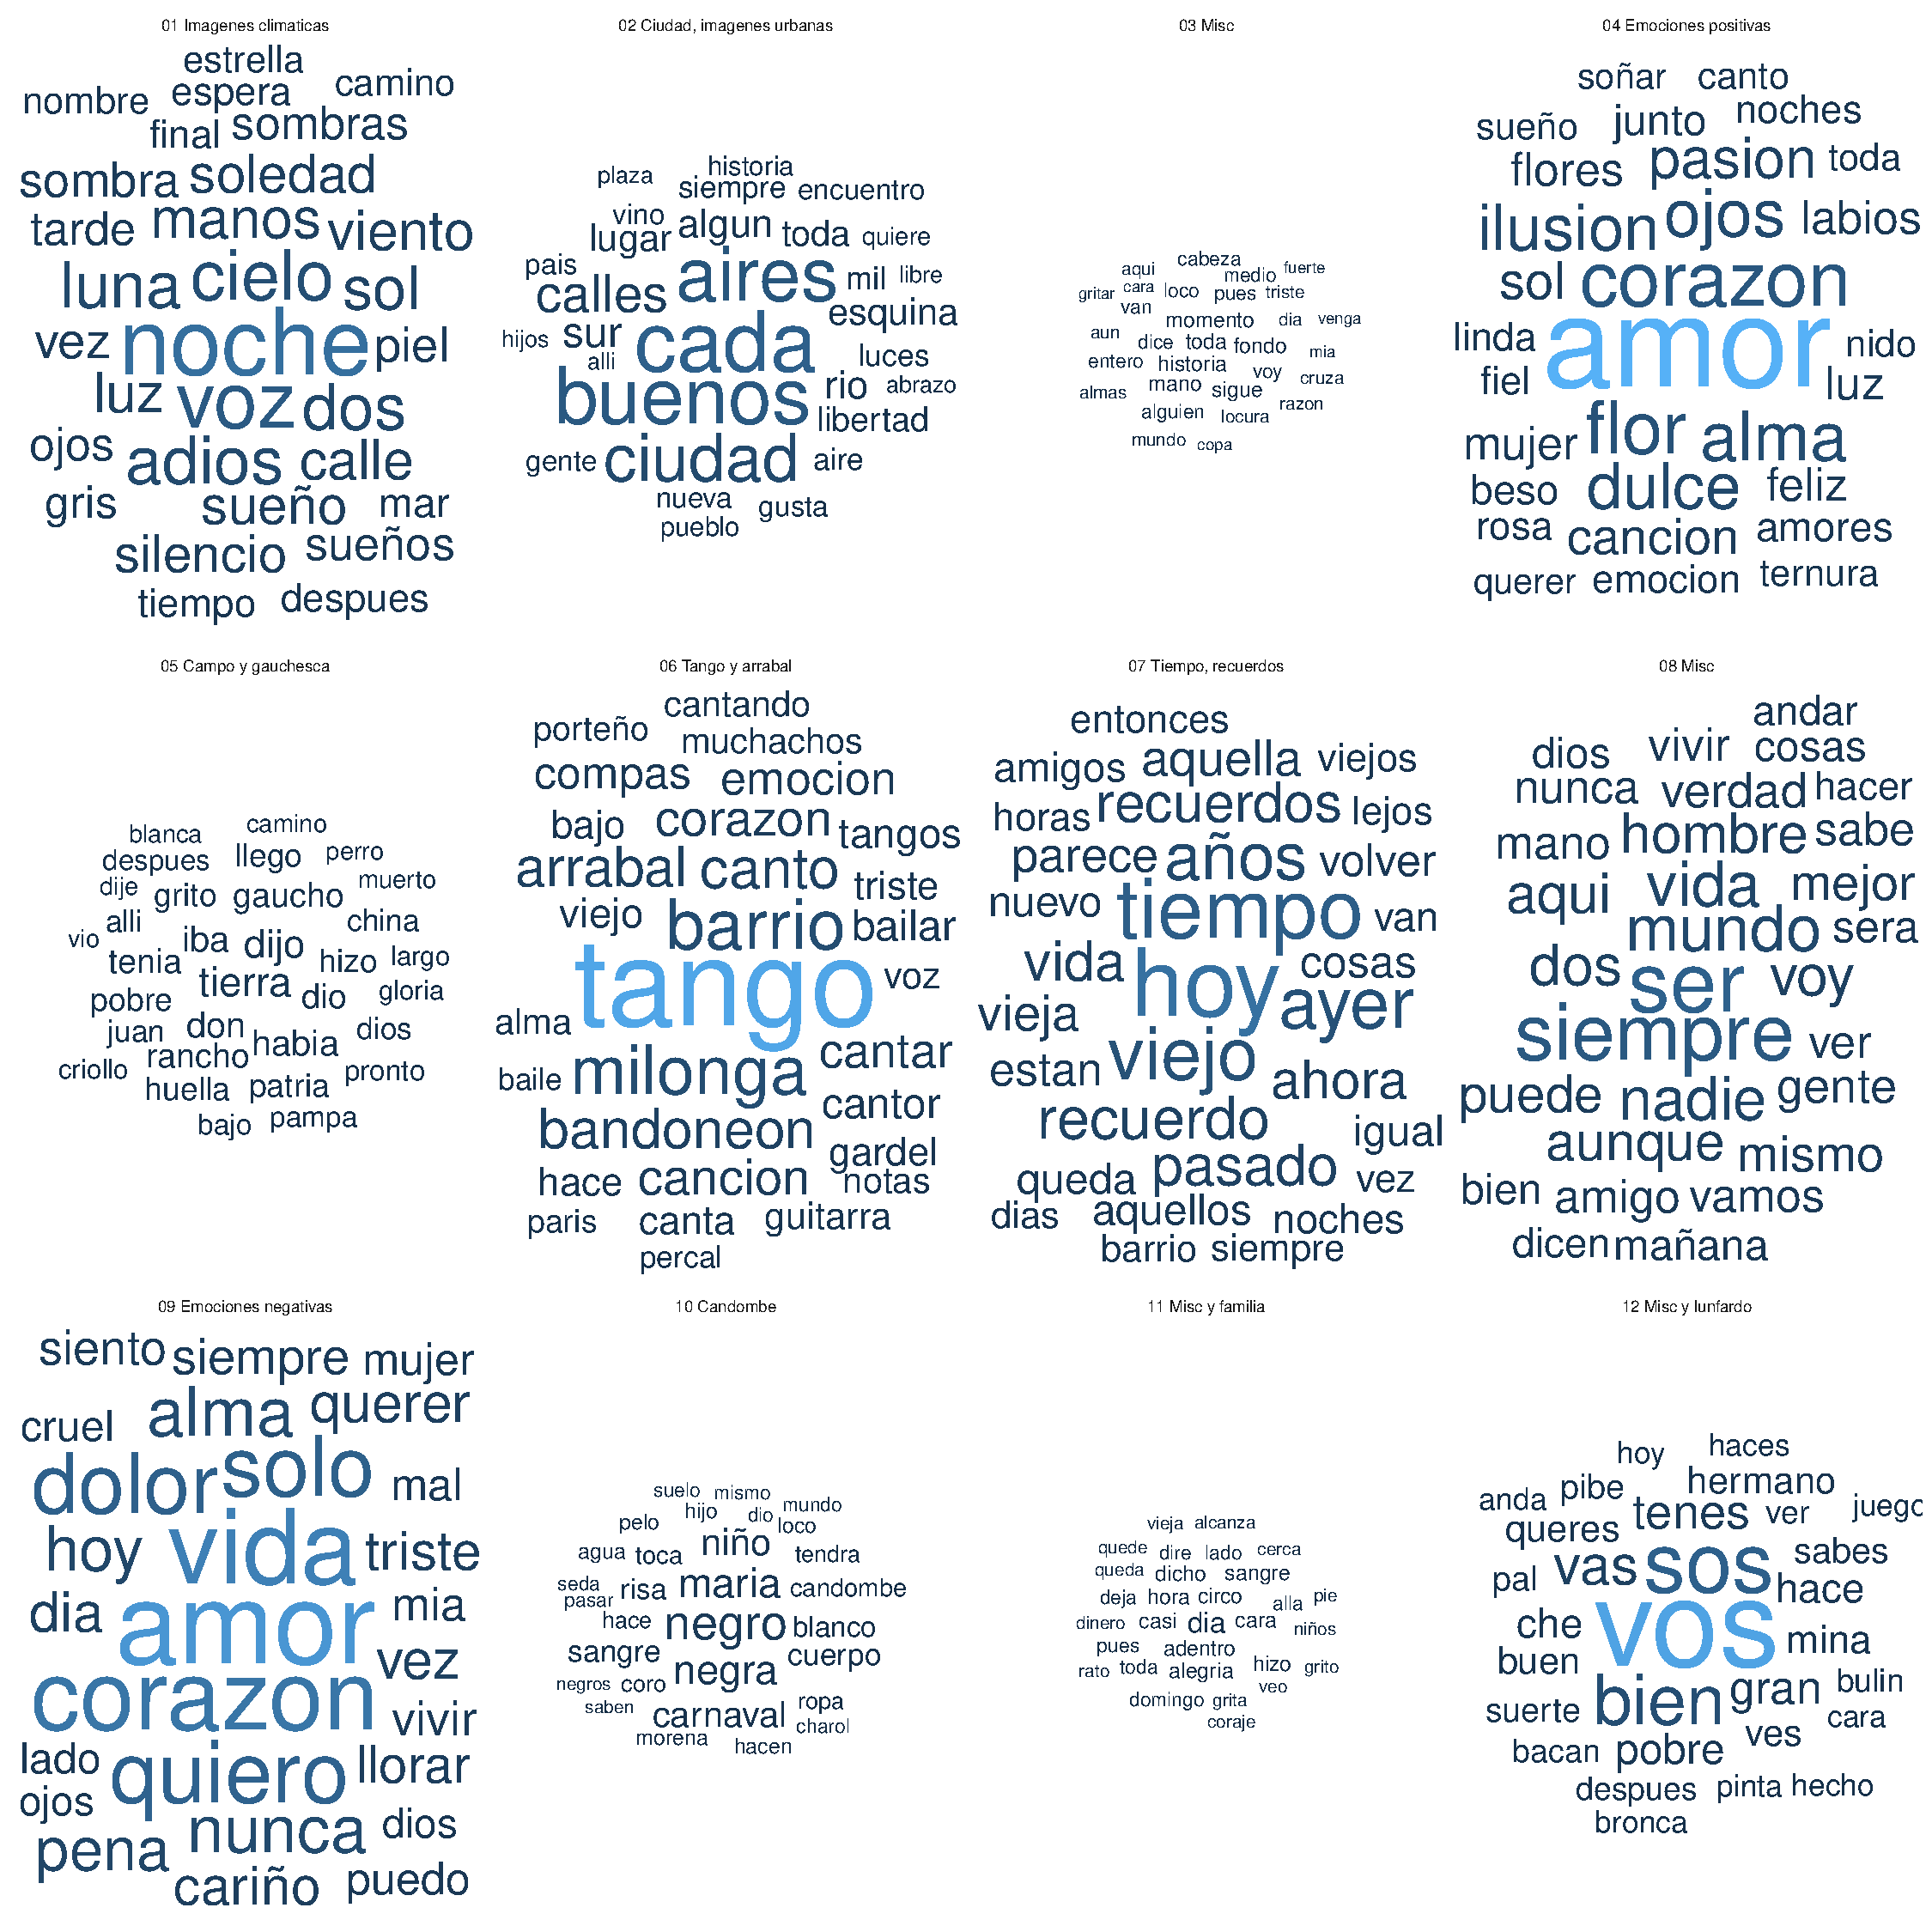
\includegraphics{Notebook_files/figure-latex/unnamed-chunk-2-1.pdf}

Puede verse que el primer tópico detectado tiene palabras como
``noche'', ``luna'', ``cielo'', ``sombras'', ``viento''. Es decir, nos
habla de imágenes naturales o climáticas.

A su vez, el segundo tópico capta el tema de la ciudad y de las imágenes
urbanas: menciona términos como ``buenos'', ``aires'', ``ciudad'',
``calles''. A su vez, el tópico 6 habla del arrabal, pero sobre todo del
tango mismo (``tango'', ``barrio'', ``arrabal'', ``canción'',
``milonga'', ``bandonéon''). El tópico 7 (``pasado'', ``recuerdo'',
``tiempo'') menciona palabras vinculadas al paso del tiempo y a la
memoria.

Los tópicos 4 y 9 contienen palabras vinculadas a las emociones. El 4
(``ilusión'', ``pasión'', ``corazón'', ``amor'') con una connotación
positiva y el 9 (``amor'', ``dolor'', ``pena'', ``triste''), negativa.

El tópico 5 y el 10 logran evidenciar tópicos de carácter ``étnico'',
por decirlo de alguna manera: el 5 con palabras como ``china'',
``gaucho'', ``tierra'', ``sangre'' capta la cuestión de la gauchesca. El
tópico 10, en cambio, (``carnaval'', ``negro'', ``morena'',
``candombe'') habla sobre el candombe y la cuestión de color.

Por último, restan cuatro tópicos. Dos de ellos (3 y 8) tienen un
carácter residual. Resultan difíciles de interpretar. No obstante, el 11
y el 12, si bien contienen muchos términos que son poco interpetables,
puede verse que el 11 (``vieja,''domingo``,''niños``) contiene palabras
vinculadas a la vida familiar y el 12, términos en lunfardo (''bulín,
``pinta'', ``che'', ``pibe). El tópico 12, también parece tener como sus
dos palabras más importantes''vos" y ``sos'', con lo cual, parece estar
captando el hecho de que se habla de forma directa a un interlocutor.

\textbf{Tabla 3. Identificación de los tópicos hallados}

\begin{longtable}[]{@{}ll@{}}
\toprule
Tópico & Etiqueta\tabularnewline
\midrule
\endhead
01 & Imagenes climaticas\tabularnewline
02 & Ciudad, imagenes urbanas\tabularnewline
04 & Emociones positivas\tabularnewline
05 & Campo y gauchesca\tabularnewline
06 & Tango y arrabal\tabularnewline
07 & Tiempo, recuerdos\tabularnewline
09 & Emociones negativas\tabularnewline
10 & Candombe\tabularnewline
11 & Misc y familia\tabularnewline
12 & Misc y lunfardo\tabularnewline
\bottomrule
\end{longtable}

Ahora bien, una vez detectados los tópicos podemos estimar para cada
documento \(d\) del corpus \(C\) que proporción presenta de cada uno de
los tópicos. A continuación se exponen la composición de tópicos de seis
tangos de tres décadas diferentes:

\textbf{Gráfico 2. Composición de tópicos según tangos, 1900-2010}

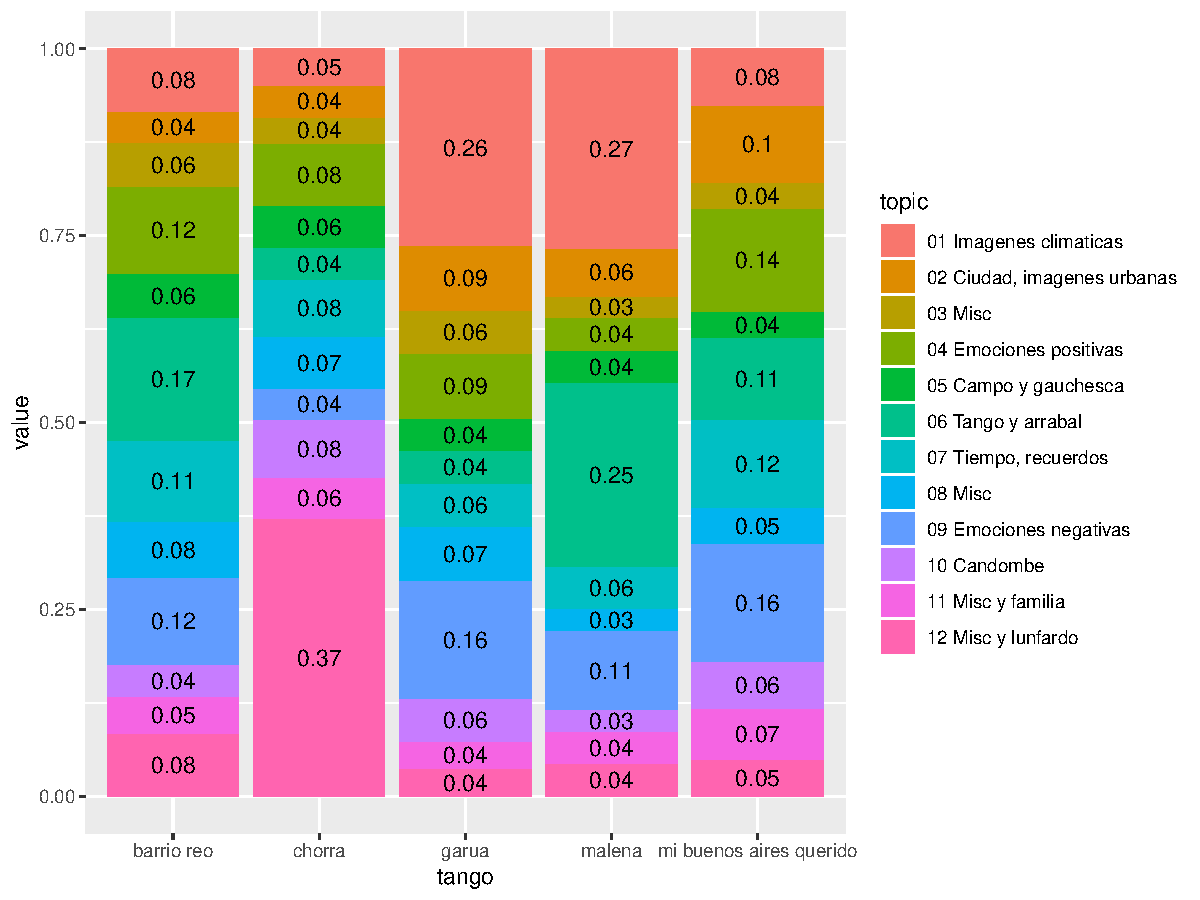
\includegraphics{Notebook_files/figure-latex/unnamed-chunk-3-1.pdf}

Así, un tango como ``Barrio Reo'', que habla de los recuerdos gratos
recuerdos del cantor al retornar a su barrio y de la tristeza que le
produce el encuentro con su deterioro (``Hoy te encuentro envejecido''),
muestra valores altos en los tópicos \emph{emociones positivas},
\emph{emociones negativas} y en el que habla sobre el \emph{tango y
arrabal}.

Al mismo tiempo, ``Chorra'', el tópico predominante es el 12. En efecto,
el tango está dedicado y dirigido a una persona (la ``chorra'' en
cuestión) y, al mismo tiempo, utiliza una buena cantidad de términos del
lunfardo (``afanaste'', ``chorra'', ``cachaban'', ``gil'').

El tango ``Garúa'' habla sobre una caminata del narrador bajo la
llovizna y pinta un cuadro lúgubre y oscuro (``sobre la calle la hilera
de focos lustra el asfalto con luz mortecina'') mientras el caminante
recuerda a la mujer que, presumiblemente se fue. Es por eso que las
\emph{emociones negativas} y las \emph{imágenes climáticas} aparecen con
fuerza en este tango.

``Malena'' nos habla (en tercera persona) de una cantante de tangos que
pasó por desamores, que parece tener la bebida fácil y que ``canta el
tango como ninguna''. Esto se corresponde con la composición de tópicos
detectada: \emph{emociones negativas}, \emph{tango y arrabal} e
\emph{imágenes climáticas} (``tono oscuro'', ``el frío del último
encuentro'', ``tus manos son palomas que sienten frío'').

Por úlimo, ``Mi Buenos Aires Querido'', nos habla de la ciudad, la
nostalgia del narrador y la esperanza del retorno. Esto se corresponde
con los tópicos detectados: \emph{ciudad}, \emph{emociones negativas},
\emph{emociones positivas} y \emph{tiempo y recuerdos}.

Al mismo tiempo, podemos analizar la evolución de cada uno de los
tópicos a lo largo de las diferentes décadas.

\textbf{Gráfico 4. Evolución de los tópicos, 1900-2010 (suavizado GAM)}

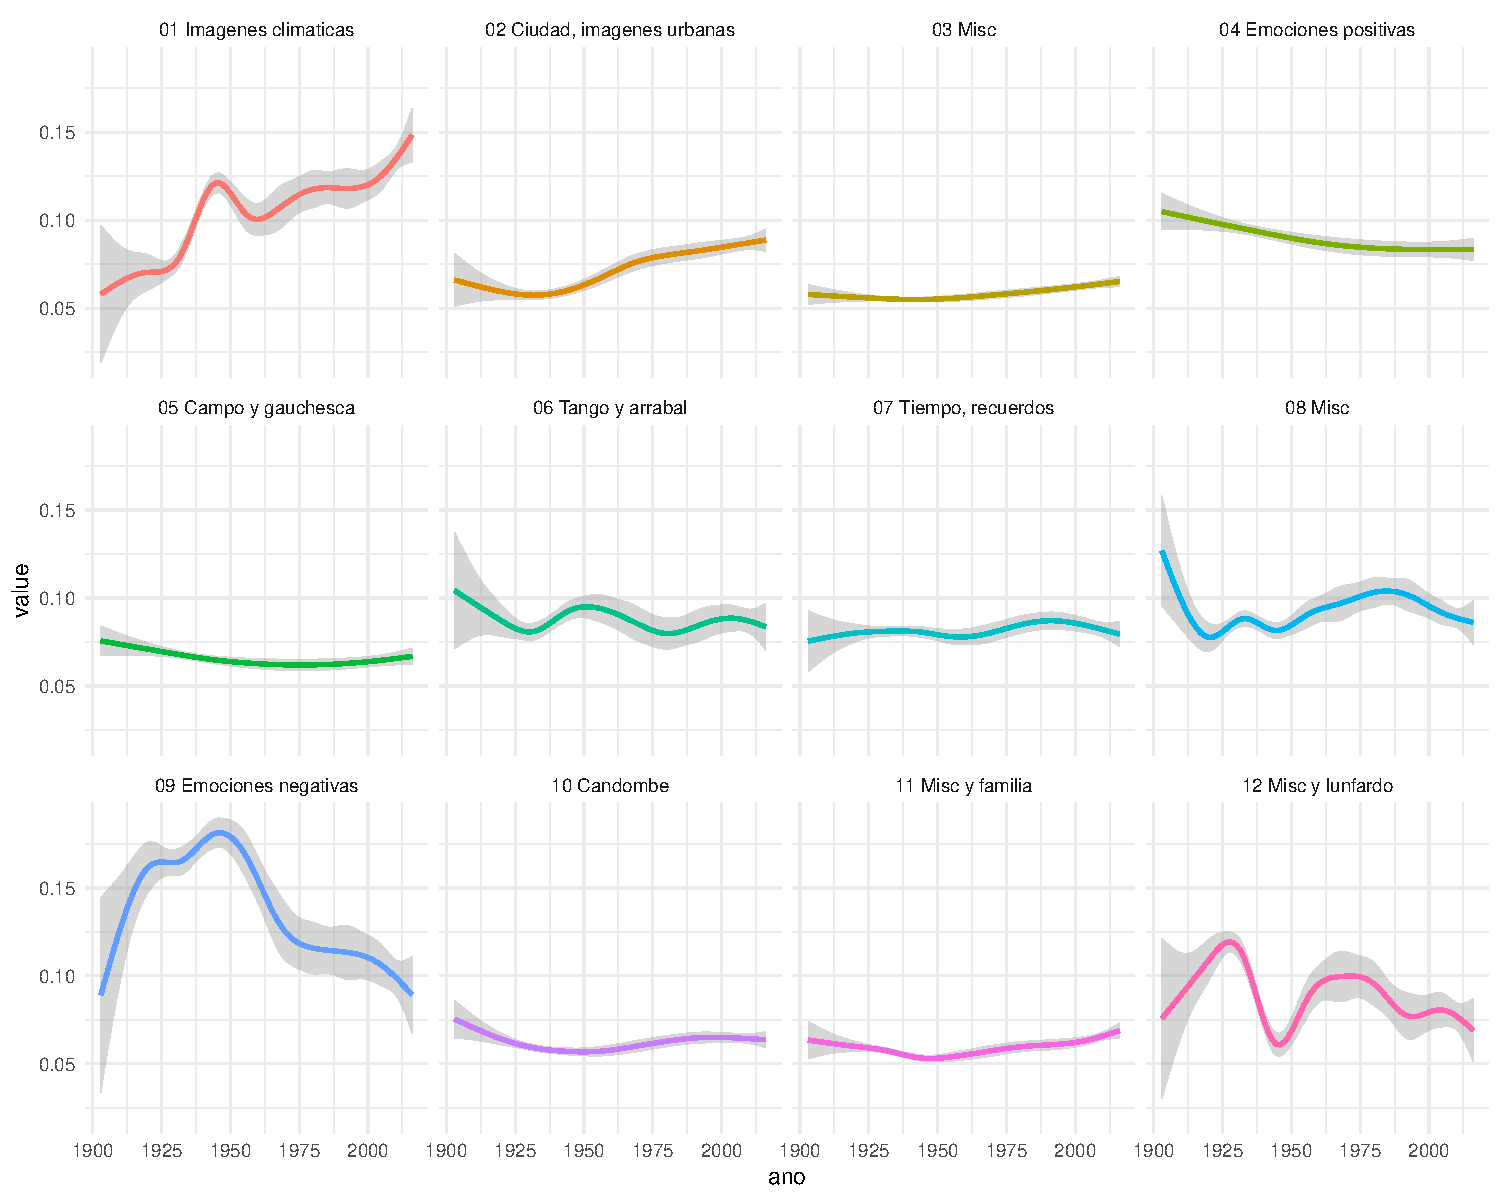
\includegraphics{Notebook_files/figure-latex/unnamed-chunk-4-1.pdf}

A partir de la evolución temporal puede verse cómo efectivamente van
modificándose los temas del tango. En primer lugar, las imágenes
naturales y climáticas ganan predominio de forma casi sostenida a lo
largo del tiempo. En mucha menor medida, el tópico vinculado a la ciudad
parece ganar cierta importancia a partir de la década del '30. También
resultan interesantes las oscilaciones que parece presentar el tema del
tango y el arrabal. Parece caer levemente hacia la década del '20 y
vuelve a incrementarse hacia los años '50, mostrando otro valle hacia
los años '70.

Pero quizás uno de los cambios más importantes es el que se observa en
los tópicos 4 y 9. En efecto, puede verse que la participación de las
emociones positivas es relativamente constante a lo largo del tiempo. En
cambio, son las emociones negativas las que muestran diferencias
fundamentales a lo largo del tiempo: muestran una tendencia al
crecimiento hasta la década del '40-'50 y luego tienden a bajar de forma
más suave.

Este punto es interesante porque toca algunas de las discusiones dentro
del campo de los estudios del tango. Así, por ejemplo Borges (2016),
planteaba que

\begin{quote}
``el tango, como hemos visto, empezó, surge de la milonga, y es al
principio un baile valeroso y feliz. Y luego, el tango va languideciendo
y entristeciéndose\ldots{}''
\end{quote}

De esta forma, puede verse que esta hipótesis parece ser corroborada por
la información construida\footnote{En el mismo texto, Borges (2016)
  discute sobre las causas de dicho cambio \textbf{DESARROLLAR}}.

Qué vinculación existe entre éstos canbios en los temas del tango u los
procesos de desarrollo del capitalismo en Argentina y a los procesos de
migración rural-urbana es una pregunta de interés para futuros pasos.

Por úlitmo, y para mostrar una última posible aplicación, podemos
calcular la composición promedio de los diferentes tópicos en cada autor
de tango. A continuación, desplegamos la composición de los cinco
autores con mayor cantidad de letras en el dataset.

\textbf{Gráfico 5. Composición de tópicos según autores, 1900-2010.
Media de la composición de las letras de tango}

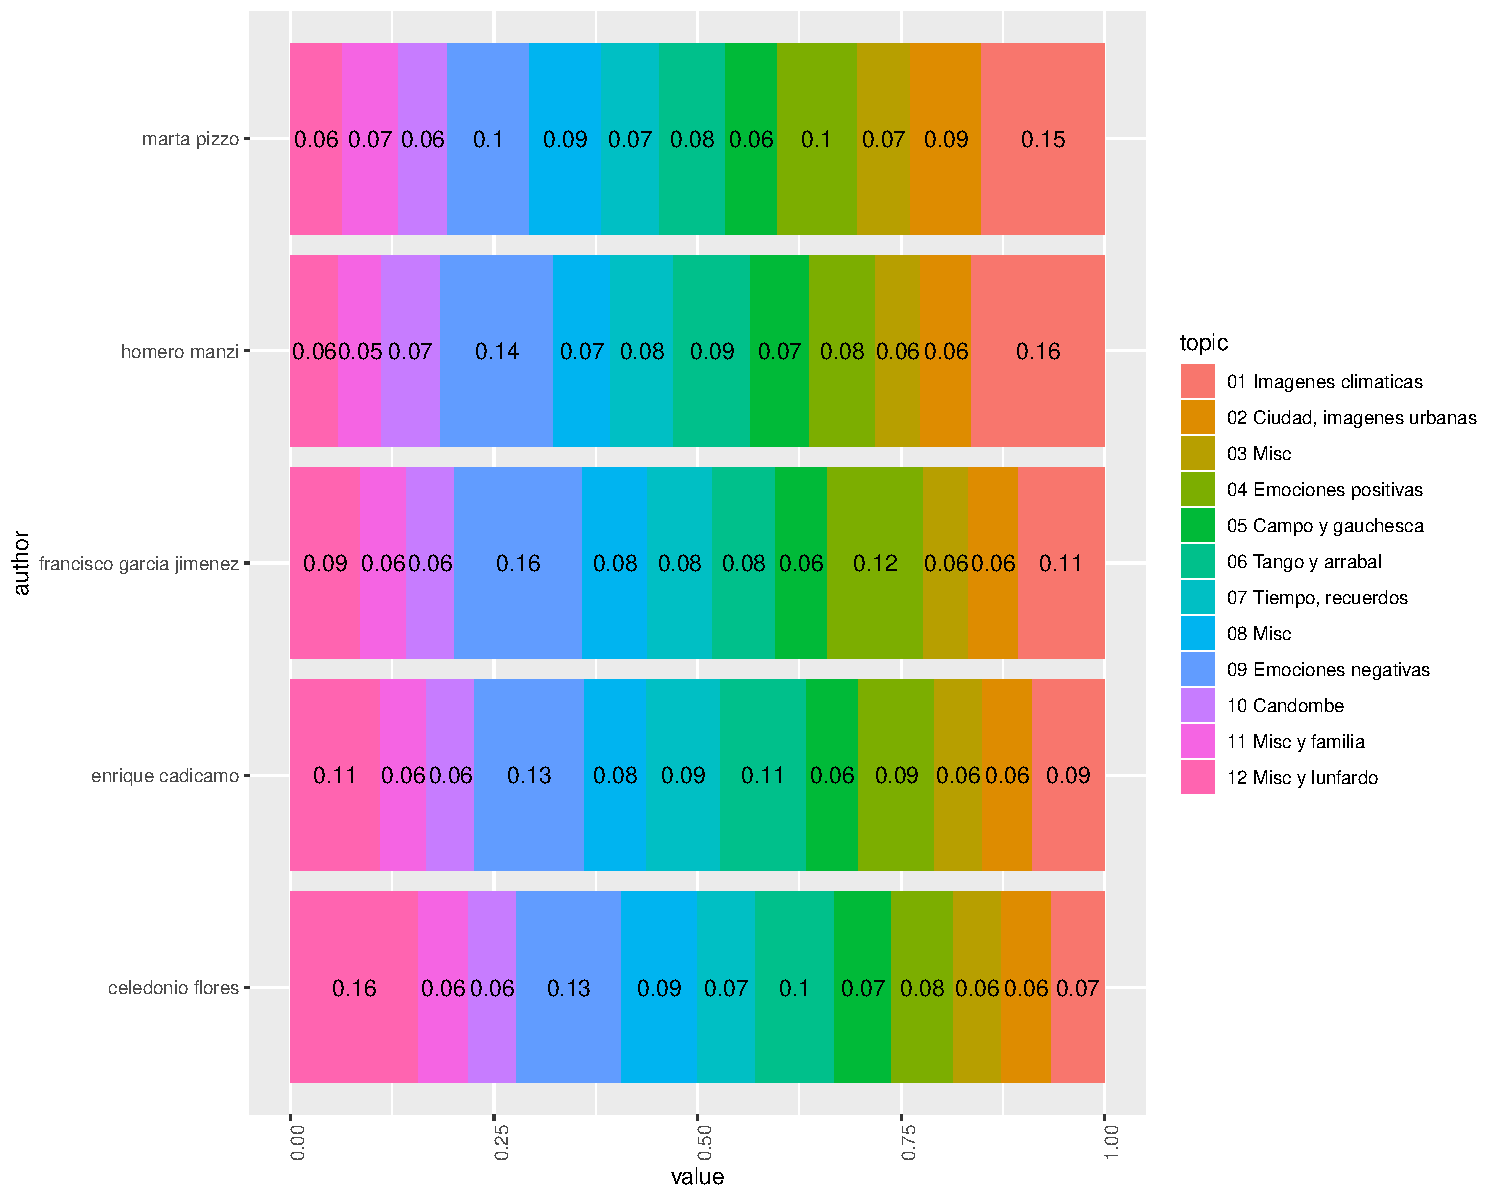
\includegraphics{Notebook_files/figure-latex/unnamed-chunk-5-1.pdf}

Así, por ejemplo, los temas predominantes de Cadícamo parecen ser el
lunfardo y las emociones negativas. Esto contrasta con Homero Manzi,
quien parece utilizar en mayor medida las imágenes climaticas (y también
las emoicones negativas).

De esta forma, podría pensarse en construir una matriz de distancias
para cada autor en función de la composición promedio de sus tópcios,
con el objetivo de encontrar autores que utilizan temas
similares.\footnote{De forma análoga podría construirse una matriz a
  nivel de tango y buscar los tangos que hablan de tópicos similares.}

\textbf{Gráfico 6. Distancias en la composición de tópicos según
autores, 1900-2010. Media de la composición de las letras de tango}

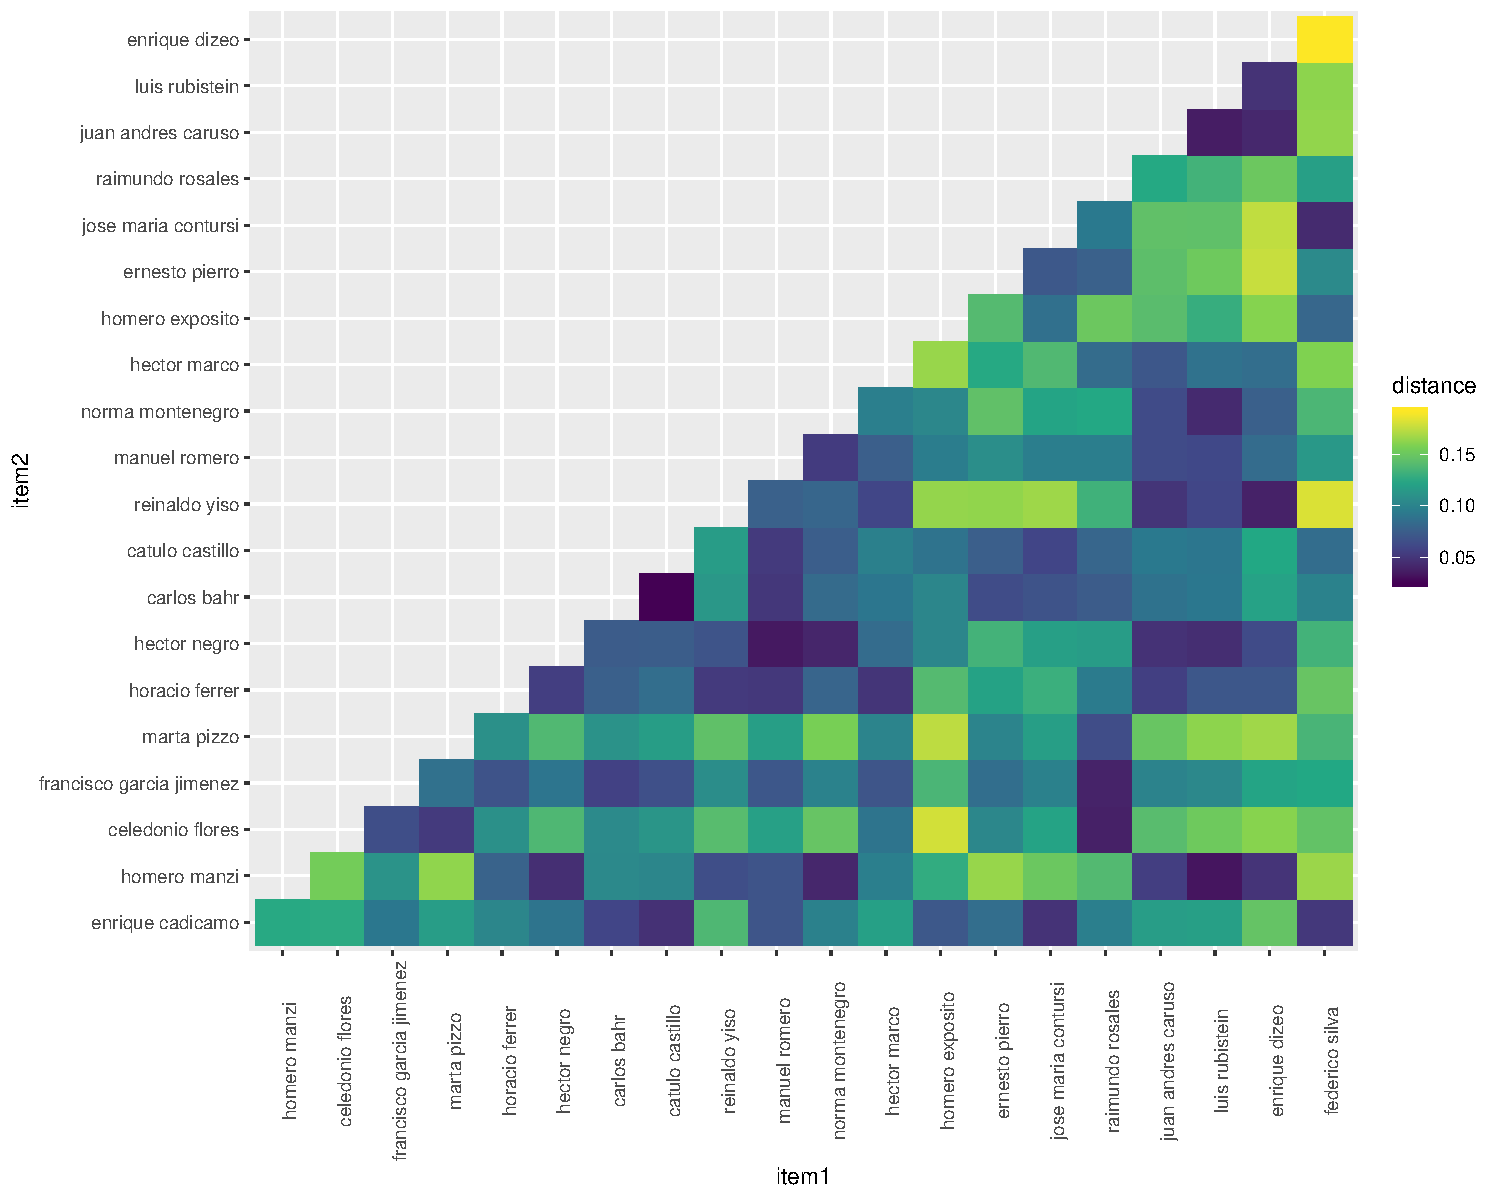
\includegraphics{Notebook_files/figure-latex/unnamed-chunk-6-1.pdf}

De esta forma, puede verse por ejemplo, que Celedonio Flores y Homero
Manzi parece ser de los que mayor similutdes tienen en relación a los
tópicos que utilizan. Algo parecido pasa con Enrique Dizeo y José María
Contursi, por un lado y con Ernesto Pierro por el otro.

\subsection{6. Resultados y discusión}\label{resultados-y-discusiuxf3n}

En el presente trabajo se buscó presentar una aproximación metodológica
posible para el análisis automático de textos. A partir de la aplicación
de una técnica de detección de tópicos (LDA) sobre un dataset de 5700
letras de tango. A su vez, se presentó un flujo de trabajo posible para
dicho análisis y se discutieron algunas técnicas para el
preprocesmaiento del texto.

De esta forma, fue posible estimar, mediante la técnica de topic
modeling LDA, los principales temas del tango. Así, el uso de emociones
positivas y negativas, imágenes de la ciudad, sobre el tango y el
arrabal, sobre el campo y la gauchesca, sobre la temporalidad y la
memoria, entre otros, aparecían como los más importantes. Al mismo
tiempo, fue posible validar los tópicos seleccionando algunos tangos y
analizando sus letras y su correspondencias con los tópicos estimados.

Quizás uno de las posibilidades analíticas más interesantes fue la de
poder analizar la evolución temporal de los tópicos y, eventualmente,
plantear hipótesis sobre la vinculación con procesos m

Finalmente, fue posible analizar las diferencias (distancias) entre los
tópicos utilizados por diferentes autores.

Ahora bien, más allá de los resultados del ejercicio propuesto (que
tienen como objetivo más mostrar un caso de uso de la herramienta que
agotar las determinaciones del objeto en cuestión), el trabajo busca
mostrar las potencialidades que este tipo de técnicas tienen para la
investigación en ciencias sociales. Particularmente, la detección de
tópicos mediante LDA ha sido utilizada en los últimos tiempos al
análisis literario (Jockers \& Mimno, 2013), al estudio de comunicados
políticos (Grimmer, 2010), al estudio de medios (Wiedemann, 2016,
DiMaggio, Nag, \& Blei (2013)), al estudio de temas en leyes y proyectos
(Gerrish \& Blei, 2012), por nombrar algunas aplicaciones relevantes.

En efecto, sus principales ventajas radican en su escalabilidad y
replicabilidad: utilizando las técnicas de análisis cualitativo de
textos ``tradicionales'', es posible lograr gran profundidad analítica
pero sobre corpus más bien pequeños o medianos y escasamente
replicables. Así, los trabajos mencionados tenían una escala más bien
pequeña: alrededor de 30 letras de tango. La excepción es el trabajo de
(Cantón, 1972). El proceso de detección de tópicos encarado en el
presente trabajo procesó y analizó una base de datos de alrededor de
6.200 letras de tango.

A su vez, el uso de técnicas automáticas de NLP no implica un
desplazamiento de los enfoques tradicionales. Un buen ejemplo es el
trabajo de (Baumer, Mimno, Guha, Quan, \& Gay, 2017), en el que se
comparan los resultados obtenidos utilizando dos métodos de análisis
sobre un mismo corpus de datos: generación de categorías utilizando la
metodología de la \emph{Grounded Theory} y detección de tópicos
utilizando LDA. Los resultados sugieren tanto una coherencia como una
complementariedad entre los resultados de ambos métodos.

\section{Bibliografía}\label{bibliografuxeda}

\section{\texorpdfstring{Anexo - Tablas con los primeros 8 términos para
estimación de tópicos con diferentes
\(k\).}{Anexo - Tablas con los primeros 8 términos para estimación de tópicos con diferentes k.}}\label{anexo---tablas-con-los-primeros-8-tuxe9rminos-para-estimaciuxf3n-de-tuxf3picos-con-diferentes-k.}

\textbf{Tabla A.1 \(k\)=15}

\begin{longtable}[]{@{}lllllllll@{}}
\toprule
topic & V1 & V2 & V3 & V4 & V5 & V6 & V7 & V8\tabularnewline
\midrule
\endhead
Topic 1 & noche & sol & tiempo & cielo & voz & dos & luna &
luz\tabularnewline
Topic 2 & vino & hombres & siempre & par & habia & dieron & flor &
invierno\tabularnewline
Topic 3 & dice & mil & muerte & paz & filo & frente & gente &
entero\tabularnewline
Topic 4 & amor & corazon & vida & quiero & dolor & alma & solo &
hoy\tabularnewline
Topic 5 & alguien & final & cada & lejos & dio & niño & pasiones &
sabia\tabularnewline
Topic 6 & siete & historia & volvio & decir & ahora & feliz & ver &
viejos\tabularnewline
Topic 7 & tango & barrio & buenos & aires & milonga & canto & cancion &
bandoneon\tabularnewline
Topic 8 & vamos & quieren & aunque & lleva & siente & oye & presencia &
primavera\tabularnewline
Topic 9 & dias & cuatro & locos & quedo & circo & van & boca &
hombres\tabularnewline
Topic 10 & lleva & gente & fuerte & rueda & sentido & quiero & romance &
cuatro\tabularnewline
Topic 11 & tierra & linda & habia & gaucho & rancho & dijo & china &
huella\tabularnewline
Topic 12 & negro & negra & maria & carnaval & libertad & sangre & niño &
hijo\tabularnewline
Topic 13 & dice & hoy & anoche & puro & rosa & hizo & lagrimas &
entro\tabularnewline
Topic 14 & mano & ahora & dire & paso & saben & traiga & media &
casi\tabularnewline
Topic 15 & vos & sos & bien & hoy & ser & siempre & vida &
vas\tabularnewline
\bottomrule
\end{longtable}

\textbf{Tabla A.2 \(k\)=13}

\begin{longtable}[]{@{}lllllllll@{}}
\toprule
topic & V1 & V2 & V3 & V4 & V5 & V6 & V7 & V8\tabularnewline
\midrule
\endhead
Topic 1 & mira & alli & dia & salio & frente & pelo & vendra &
edad\tabularnewline
Topic 2 & paso & ser & llevo & partida & loco & años & bandera &
fuerte\tabularnewline
Topic 3 & sangre & medio & dice & viene & tumba & vez & cuerpo &
quedan\tabularnewline
Topic 4 & noche & voz & tiempo & cielo & luna & dos & sol &
calle\tabularnewline
Topic 5 & tierra & dijo & don & viejo & tenia & gaucho & grito &
rancho\tabularnewline
Topic 6 & tango & barrio & buenos & aires & milonga & viejo & bandoneon
& arrabal\tabularnewline
Topic 7 & vamos & dias & loco & cuatro & libertad & viva & año &
dale\tabularnewline
Topic 8 & amor & vida & corazon & solo & quiero & dolor & hoy &
alma\tabularnewline
Topic 9 & pues & trabajo & quedo & tras & vida & pies & vio &
algun\tabularnewline
Topic 10 & amor & flor & ojos & corazon & alma & dulce & cancion &
ilusion\tabularnewline
Topic 11 & siempre & ser & vida & mundo & nadie & cosas & hombre &
mismo\tabularnewline
Topic 12 & negro & sangre & negra & maria & niño & carnaval & risa &
cuerpo\tabularnewline
Topic 13 & vos & sos & bien & hoy & vas & tenes & gran &
pobre\tabularnewline
\bottomrule
\end{longtable}

\textbf{Tabla A.1 \(k\)=10}

\begin{longtable}[]{@{}lllllllll@{}}
\toprule
topic & V1 & V2 & V3 & V4 & V5 & V6 & V7 & V8\tabularnewline
\midrule
\endhead
Topic 1 & amor & corazon & alma & flor & ilusion & ojos & pasion &
dulce\tabularnewline
Topic 2 & cada & buenos & aires & calle & ciudad & esquina & calles &
van\tabularnewline
Topic 3 & noche & voz & cielo & dos & adios & luna & sol &
manos\tabularnewline
Topic 4 & tierra & gran & don & gloria & alli & huella & grito &
gaucho\tabularnewline
Topic 5 & tango & barrio & milonga & canto & bandoneon & arrabal &
cancion & cantar\tabularnewline
Topic 6 & pobre & triste & dia & noche & aquella & madre & pena &
dio\tabularnewline
Topic 7 & amor & vida & corazon & quiero & solo & dolor & nunca &
alma\tabularnewline
Topic 8 & ser & siempre & mundo & nadie & hombre & voy & aqui &
mejor\tabularnewline
Topic 9 & hoy & tiempo & ayer & vida & viejo & años & recuerdo &
vez\tabularnewline
Topic 10 & vos & sos & bien & vas & tenes & gran & hace &
che\tabularnewline
\bottomrule
\end{longtable}

\textbf{Tabla A.1 \(k\)=5}

\begin{longtable}[]{@{}lllllllll@{}}
\toprule
topic & V1 & V2 & V3 & V4 & V5 & V6 & V7 & V8\tabularnewline
\midrule
\endhead
Topic 1 & triste & vida & ojos & dia & pobre & alma & pena &
noche\tabularnewline
Topic 2 & dos & noche & voz & tiempo & cielo & sol & adios &
cada\tabularnewline
Topic 3 & tango & viejo & barrio & buenos & aires & milonga & canto &
cancion\tabularnewline
Topic 4 & amor & corazon & vida & solo & quiero & dolor & hoy &
nunca\tabularnewline
Topic 5 & vos & bien & sos & ser & vas & siempre & hombre &
hoy\tabularnewline
\bottomrule
\end{longtable}

\hypertarget{refs}{}
\hypertarget{ref-asuncion}{}
Asuncion, A., Welling, M., Smyth, P., \& Teh, Y. W. (2009). On smoothing
and inference for topic models. \emph{Proceedings of the twenty-fifth
conference on uncertainty in artificial intelligence}, 27--34. Retrieved
from \url{http://dl.acm.org/citation.cfm?id=1795114.1795118}

\hypertarget{ref-baumer}{}
Baumer, E., Mimno, D., Guha, S., Quan, E., \& Gay, G. (2017). Comparing
grounded theory and topic modeling: Extreme divergence or unlikely
convergence? \emph{Journal of the Assosiation for Information Science
and Technology}, \emph{6}(68). Retrieved from
\url{https://mimno.infosci.cornell.edu/papers/baumer-jasist-2017.pdf}

\hypertarget{ref-blei1}{}
Blei, D. (2012). Probabilistic topic models. \emph{Communications of the
ACM}, \emph{55}(4).

\hypertarget{ref-borges}{}
Borges, J. L. (2016). \emph{El tango. cuatro conferencias}.
Sudamericana.

\hypertarget{ref-canton}{}
Cantón, D. (1972). \emph{Gardel, ¿a quién le cantás?} De la Flor.

\hypertarget{ref-chang}{}
Chang, J., Boyd-Graber, J., Wang, C., Gerrish, S., \& Blei, D. M.
(2009). Reading tea leaves: How humans interpret topic models.
\emph{Neural information processing systems}. Retrieved from
\url{docs/nips2009-rtl.pdf}

\hypertarget{ref-blei2}{}
DiMaggio, P., Nag, M., \& Blei, D. (2013). Exploiting affinities between
topic modeling and the sociological perspective on culture: Application
to newspaper coverage of u.S. government arts funding. \emph{Poetics},
\emph{41}(6). Retrieved from
\url{https://www.sciencedirect.com/science/article/pii/S0304422X13000661}

\hypertarget{ref-gasparri1}{}
Gasparri, J. (2011). Che varón, masculinidades en las letras de tango.
\emph{Revista Caracol}, (2).

\hypertarget{ref-geertz}{}
Geertz, C. (1974). Deep play: Notes on the balinese cockfight. In
\emph{The interpretation of cultures} (pp. 412--453). New York: Basic
Books.

\hypertarget{ref-blei3}{}
Gerrish, S., \& Blei, D. M. (2012). How they vote: Issue-adjusted models
of legislative behavior. In F. Pereira, C. J. C. Burges, L. Bottou, \&
K. Q. Weinberger (Eds.), \emph{Advances in neural information processing
systems 25} (pp. 2753--2761). Retrieved from
\url{http://papers.nips.cc/paper/4715-how-they-vote-issue-adjusted-models-of-legislative-behavior.pdf}

\hypertarget{ref-grimmer2}{}
Grimmer, J. (2010). A bayesian hierarchical topic model for political
texts: Measuring expressed agendas in senate press releases.
\emph{Political Analysis}, \emph{18}(1).

\hypertarget{ref-grimmer}{}
Grimmer, J., \& Stewart, M. (2013). Text as data: The promise and
pitfalls of automatic content analysis methods for political texts.
\emph{Political Analysis}, (2013). Retrieved from
\url{http://pan.oxfordjournals.org/}

\hypertarget{ref-hassani}{}
Hassani, A., Iranmanesh, A., \& Mansouri, N. (2019). \emph{Text mining
using nonnegative matrix factorization and latent semantic analysis}.

\hypertarget{ref-fang}{}
Hsieh, H.-F., \& Shannon, S. E. (2005). Three approaches to qualitative
content analysis. \emph{Qualitative Health Research}, \emph{15}(9).

\hypertarget{ref-jockers}{}
Jockers, M., \& Mimno, D. (2013). Significant themes in 19th-century
literature. \emph{Poetics}, \emph{41}(6).

\hypertarget{ref-lopez_i}{}
López, I. (2010). Morochas, milongueras y percantas. representaciones de
la mujer en las letras de tango. \emph{Espéculo. Revista de Estudios
Literarios.}, (45). Retrieved from
\url{http://webs.ucm.es/info/especulo/numero45/mutango.html}

\hypertarget{ref-marchese1}{}
Marchese, M. (2007). Tango. el lenguaje quebrado del desarraigo.
\emph{Revista Latinoamericana de Estudios Del Discurso}, \emph{6}(2).

\hypertarget{ref-mimno}{}
Mimno, D., Wallach, H., Talley, E., Leenders, M., \& McCallum, A.
(2011). Optimizing semantic coherence in topic models. \emph{Empirical
methods on natural language processing}. Retrieved from
\url{https://mimno.infosci.cornell.edu/papers/mimno-semantic-emnlp.pdf}

\hypertarget{ref-mitchell}{}
Mitchell, R. (2015). \emph{Web scraping with python: Collecting data
from the modern web}. O'Reilly Media, Inc.

\hypertarget{ref-reynoso1}{}
Reynoso, C. (2007). El lado oscuro de la descripción densa.
\emph{Anthropologika. Revista de Estudio E Investigaciones En
Antropología}, \emph{1}(1).

\hypertarget{ref-wind}{}
Wiedemann, G. (2016). \emph{Text mining for qualitative data analysis in
the social sciences. a study on democratic discourse in germany}.
\url{https://doi.org/10.1007/978-3-658-15309-0}

\hypertarget{ref-willenpart}{}
Willenpart, L. (2011). El tango: Temas y motivos. \emph{Verba
Hispánica}, \emph{9}(1).


\end{document}
